\chapter{State Pattern}
Nachfolgend wird das eingesetzte Design Pattern State erläutert.
\section{Context, Interface und Concrete Klassen}
In der vorliegenden Ampelschaltung werden zwei State Patterns verwendet. Zudem wird beim Input und Output sich eines Interfaces bedient, welches Polymorphie zulässt. Das heißt, je nachdem ob Hardware angeschlossen ist, werden die Hardware oder Software Klassen verwendet. Näheres dazu wird in dem Kapitel \glqq Wechsel zwischen Hardware- und Softwarebetrieb\grqq{} beschrieben. Das hierarchisch höhere State Pattern besteht aus der Kontextklasse \glqq TrafficLight\grqq{}, dem Interface \glqq state\grqq{} und den Concrete Klassen \glqq flashing\grqq{} und \glqq active\grqq{}. Je nach Benutzereingabe verweist der Zeiger vom Typ \glqq state\grqq{} auf eine Instanz der Klasse \glqq flashing\grqq{} oder \glqq active\grqq{}. Wird die Handle Funktion des Interfaces aufgerufen, ist die Ampel entweder im konkreten Zustand \glqq in Betrieb\grqq{} oder \glqq außer Betrieb\grqq{}. Fordert der Benutzer ein Wechsel des Betriebsmodus, so ist der nächste Zustand der jeweils andere Betriebsmodus. Das zweite State Pattern wechselt zwischen den Farbzuständen. Dieses State Pattern besteht entweder aus der Kontextklasse \glqq flashing\grqq{} oder \glqq active\grqq{}, dem Interface \glqq LightControl\grqq{} und den Concrete Klassen (\glqq Off\grqq{}, \glqq Red\grqq{}, \glqq RedAmber\grqq{}, \glqq Amber\grqq{},  \glqq Green\grqq{}). Die Klasse  \glqq active\grqq{} ruft die Funktionen \glqq nextstate\grqq{} des Interfaces auf, damit die Ampelfarben durchgeschaltet werden. Im außer Betrieb Zustand wechselt der Farbzustand der Ampel zwischen Off und Amber.

\section{Singleton}
Das Singleton Design Pattern hilft in der objektorientierten Programmierung dem Entwickler mit vielfachen Vorlagen das Lösen von Programmieraufgaben. Es ist sehr leistungsfähig und gehört zu der Kategorie der Erzeugungsmuster unter den Design Pattern. Der Ausdruck Singleton wird oftmals als \glqq Einzelstück\grqq{} betitelt. Dieses Synonym bildet sehr gut die Funktion einens Singeltons ab, da die Aufgabe darin besteht nicht mehr als ein Objekt einer Klasse zu erstellen. Wurde mit der Klasse über das Singleton Pattern nur eine Instanz der Klasse erzeugt, sorgt es auch dafür, dass es ledlich bei dieser einen Instanz der Klasse bleibt. Oftmals dient eine Funktion, wie \texttt{GetInstance} dafür, dass nur eine Instance der Klasse erstellt wird.\\
\\
Im Bezug auf die Ampelsteuerung wurde das Singleton Pattern in elf unterschiedlichen Klassen verwendet. Diese lauten wie folgt:

\begin{itemize}
	\item active.h
	\item flashing.h
	\item Red.h
	\item Amber.h
	\item RedAmber.h
	\item Green.h
	\item Off.h
	\item SoftwareInput.h
	\item SoftwareOutput.h
	\item HardwareInput.h
	\item HardwareOutput.h
\end{itemize}

Da der Aufbau in jeder Klasse identisch ist, folgt die Erläuterung im Code nun am Beispiel der Klasse \texttt{Red.h}.\\

\begin{figure}[H] 
	\centering
	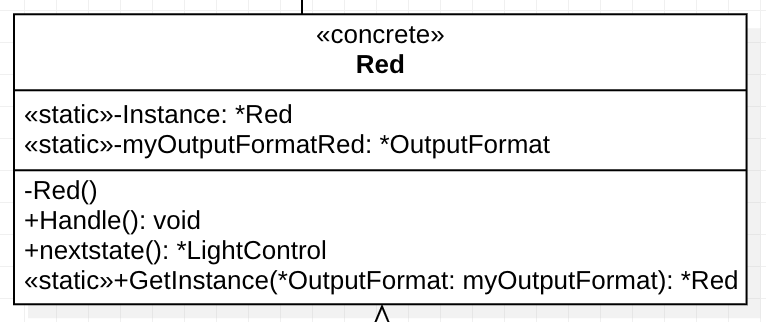
\includegraphics[width=0.5\textwidth]{images/07.png}
	\caption{Singleton Patten am Beispiel der Red.h Klasse \protect \\ Quelle: Eigene Darstellung }
	\label{fig:grafik7}
\end{figure}

In der \autoref{fig:grafik7} sind die Funktionen und Instanzen der Red.h Klasse zu sehen, welche mit Hilfe des Singleton Pattern implementiert wurde. Das Schlüsselwort \texttt{static} bedeutet einmal, dass die als \texttt{static} deklarierte Variable oder Funktion ihren Wert innerhalb zwischen Aufrufen behält und andermal, dass eine globale statische Variable oder Funktion nur in der Datei \glqq gesehen\grqq{} wird, in der sie deklariert wurde. Um das Singleton Pattern nutzen zu können, wird die statische Instanz und die Funktion \texttt{GetInstance} benötigt. Die Funktion \texttt{GetInstance} hat die Aufgabe, bei jedem Aufruf eine Instance zu erzeugen (siehe \autoref{codeauszug:red.h1}). \\

\begin{lstlisting}[style=myC,caption={Red.cpp - Singleton in der Klasse Red},label={codeauszug:red.h1},captionpos=b]
	...
	Red *Red::Instance = NULL;
	
	Red *Red::GetInstance(OutputFormat *myOutputFormat)
	{
		myOutputFormatRed = myOutputFormat; 
		if (Instance == NULL)
		{
			Instance = new Red();
		}
		return Instance;
	}
	...
\end{lstlisting}

Wie in Zeile 2 zu erkennen ist, wird die Instanz der Klasse immer auf \texttt{NULL} deklariert. In Zeile 4 der cpp-Datei wird ist die Implementierung der Funktion \texttt{GetInstance} zu sehen. Innerhalb dieser Funktion wird der übergebene Parameter \texttt{myOutputFormat} der Klasse Red zugeweisen. Folgend findet eine \texttt{if} Überprüfung statt, ob es schon eine Instance der Klasse Red.h gibt. Wenn nicht, wird in Zeile 9 eine neue Instanz der Klasse Red.h erzeugt. Anschließend besitzt die Funktion \texttt{GetInstance} als \texttt{return}-Wert die erzeugte Instanz. Wichtig ist es, dass die statische Instanz als \texttt{private} und die Funktion \texttt{GetInstance} als \texttt{public}.

\chapter{Hardwarezugriff - GPIO}
Der Hardwarezugriff erfolgt über drei Klassen. Die untergeordnete Klasse \texttt{GPIO} greift dabei direkt auf die Register des Mikrocontrollers zu und steuert somit sämtliche Hardwarezugriffe. Die zwei übergeordneten Klassen \texttt{UserLEDs} und \texttt{UserButtons} greifen dann auf die Klasse \texttt{GPIO} zu und steuern diese. Übergeordnet heißt hier jedoch nicht, dass es sich um Oberklassen einer Vererbung handelt. Die hier herrschende Beziehung ist eine Aggregation. Außer zu diesen beiden Klassen hat die \texttt{GPIO}-Klasse keine weiteren Verbindungen. Eine Hardwareansteuerung kann somit nur durch die beiden genannten übergeordneten Klassen durchgeführt werden.\\
\\
Nun wird etwas genauer auf die die \texttt{GPIO}-Klasse eingegangen. Sie ist wie folgt aufgebaut:

\begin{figure}[H] 
	\centering
	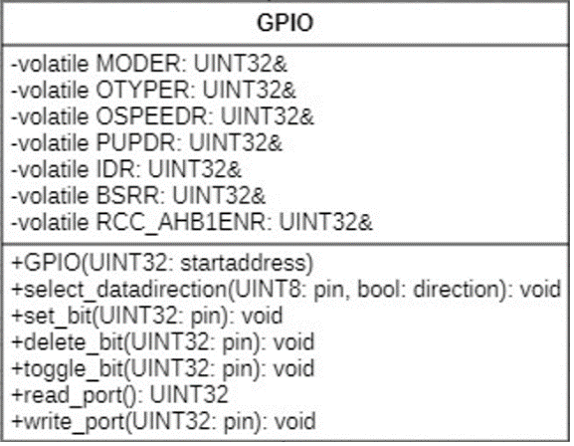
\includegraphics[width=0.5\textwidth]{images/04.png}
	\caption{GPIO Klasse \protect \\ Quelle: Eigene Darstellung}
	\label{fig:grafik4}
\end{figure}

Alle Attribute dieser Klasse sind als \glqq private\grqq{} gekennzeichnet. Das liegt daran, dass es sich bei den Attributen um Zeiger handelt, mit welchen man auf die GPIO-Register des Mikrocontrollers zugreifen kann. Hier wird das Prinzip des Information Hidings angewendet, um zu verhindern, dass die Register von außen manipuliert werden könnten. Weiterhin wird den Attributen das Schlüsselwort volatile vorangestellt. Dieses gibt dem Compiler die Information, dass sich der Inhalt auf den die Zeiger zeigen, ändern kann, auch wenn das Programm nicht schreibend darauf zugreift.\\
\\
Der Konstruktor der Klasse konfiguriert einen GPIO-Port. Ihm muss lediglich die Startadresse des gewünschten Ports übergeben werden. Diese Startadresse kann dem Datenblatt auf Seite 53 entnommen werden. Auf Basis der Startadresse adressiert dieser dann die benötigten Register. Weiterhin wird dort das Clock Signal des ausgewählten Ports aktiviert.
Über die Methode \texttt{select\_datadirection()} kann dann für jeden Pin des Ports einzeln ausgewählt werden ob, dieser als Input oder als Output fungieren soll. Dazu muss der Methode nur die Pinnummer und die Art des GPIOs übergeben werden.
Mit \texttt{set\_bit()} kann ein ausgewählter Output gesetzt werden. Dazu muss lediglich die Pinnummer bekannt sein. \texttt{delete\_bit()} macht genau das Gegenteil. Dort wird ein Output zurückgesetzt. \texttt{toggle\_bit()} vereint beide Methoden. Dort wird der Status des Outputs abgefragt und danach umgekehrt.
Mit \texttt{read\_port()} werden die Zustände jedes einzelnen Pins des gesamten Ports gelesen und als 32-Bit Wert zurückgeben. Bei der Ausführung von \texttt{write\_port()} hingegen, wird der gesamte Port beschrieben. Wirksam ist der Schreibzugriff jedoch nur auf definierte Outputs.\\
\\
Nun wird auf die Klasse \glqq UserLEDs\grqq{} betrachtet. Das dazugehörige Klassendiagramm kann folgender Abbildung entnommen werden: \\

\begin{figure}[H] 
	\centering
	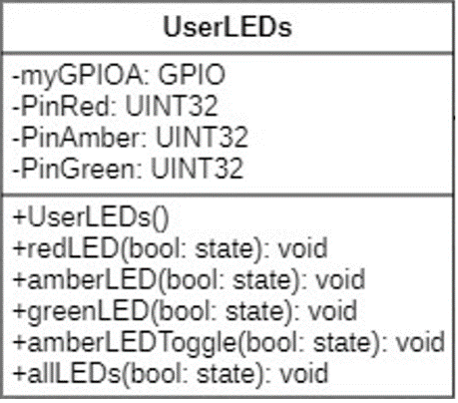
\includegraphics[width=0.35\textwidth]{images/05.png}
	\caption{UserLEDs Klasse \protect \\ Quelle: Eigene Darstellung}
	\label{fig:grafik5}
\end{figure}

Auch hier sind alle Attribute als private definiert, um das Information Hiding zu waren. Das erste Attribut ist eine Instanz der \texttt{GPIO}-Klasse. Es dient als Schnittstelle zur Ansteuerung der Pins, an welchen die LEDs angeschlossen sind. In den restlichen drei Attributen werden die jeweiligen Pinnummern der LEDs hinterlegt. Dies erfolgt im Konstruktor über eine Initialisierungsliste. Danach wird dort noch, über die \texttt{select\_datadirection()}-Methode der \texttt{GPIO}-Klasse festgelegt, dass es sich bei den vorliegenden Pins um Outputs handelt. Mit den restlichen Methoden werden dann die LEDs angesteuert. Ihnen muss lediglich der gewünschte Zustand übergeben werden.\\
\\
Zuletzt wird die Klasse \texttt{UserButtons} betrachtet. Auch hier wird ein UML Klassendiagramm zur Erläuterung herbeigezogen:\\

\begin{figure}[H] 
	\centering
	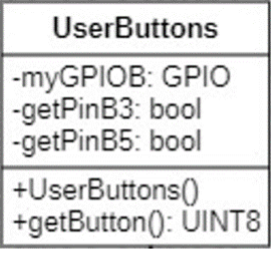
\includegraphics[width=0.2\textwidth]{images/06.png}
	\caption{UserButtons Klasse \protect \\ Quelle: Eigene Darstellung }
	\label{fig:grafi6}
\end{figure}

Dort wird auch wieder eine private Instanz der Klasse \texttt{GPIO} erstellt. Damit können die Buttons abgefragt werden. Weiterhin existieren zwei private Methoden, welche den Status des jeweiligen Buttons zurückgeben. Sie werden in der Methode \texttt{getButton()} aufgerufen. Dort erfolgt eine Entprellung. Dazu wird der Wert zunächst ein erstes Mal abgefragt. Danach wird 3000 Schleifendurchgänge gewartet und der Status erneut abgefragt. Liefern beide Abfragen das gleiche Ergebnis, so wird der Wert übernommen. Andernfalls wird die Entprellung erneut durchgeführt. Wie im Klassendiagramm zu sehen hat die Methode einen Rückgabewert vom Datentyp \texttt{UINT8}, dies entspricht einem 8 Bit Charakter. Je nachdem, welcher Button nun gedrückt wird, wird ein bestimmter Rückgabewert zurückgegeben. Eine Auflistung aller möglichen Rückgabewerte kann folgender \autoref{tab:Rueckgabe} entnommen werden:\\

\begin{table}[H]
	\centering
	\begin{tabular}[H]{c|c}
	Welche Buttons gedrückt? & Rückgabewert \\
	\hline
	Keiner & O \\
	Nur Button an B3 (D3) & B \\
	Nur Button an B5 (D4) & F \\
	Beide Buttons &  X \\
	\end{tabular}
	\caption{Rückgabewerte Buttons}
	\label{tab:Rueckgabe}
\end{table}

\chapter{Wechsel zwischen Hardware- und Softwarebetrieb}
Nachstehend wird die Umsetzung der Wechsels zwischen Hardware- und Softwarebetrieb erläutert.
\section{Definition}
Wie bereits erwähnt, soll es dem Anwender möglich sein, die Ampelsteuerung sowohl mit Hardware, als auch komplett ohne Hardware nutzen zu können. Um die beiden Fälle näher zu erläutern, wird der Hardware- und Softwarebetrieb im Folgenden konkret spezifiziert.

\begin{itemize}
	\item \textbf{Hardwarebetrieb:} Der Programmcode der Ampelsteuerung wird auf das Nucleo Board geflasht und auf diesem ausgeführt. Die Nutzereingabe erfolgt über zwei an das Board angeschlossenen Taster. Die Ausgabe der Ampelfarben erfolgt über die drei angeschlossenen LEDs.
	\item \textbf{Softwarebetrieb:} Das Programm der Ampelsteuerung wird auf dem PC ausgeführt. Die Nutzereingabe erfolgt über die Tastatur. Die Tasten \glqq F\grqq\:und \glqq B\grqq\:repräsentieren die beiden Hardwaretaster. Die Taste \glqq X\grqq\:steht für das Betätigen beider Taster gleichzeitig. Das Einlesen der Tastatureingaben erfolgt über den Eingabestream \texttt{cin}, die Ausgabe der Ampelfarben über den Ausgabestream \texttt{cout} in der Kommandozeile.
\end{itemize}

\section{Umsetzung}
Ob die Ampelsteuerung im Hardware- oder Softwarebetrieb arbeitet, wird über Pointer bestimmt, welche in der \:\texttt{main.cpp}\: des Programmes angelegt und bis zur relevanten Stelle im Programmcode durch alle Klassen übergeben werden. Ob die Pointer für den Hardware- oder Softwarebetrieb initialisiert werden, wird wiederum über eine Präprozessoranweisung festgelegt, welche der Nutzer setzen oder auskommentieren kann. Dies ist in \autoref{codeauszug:HWSW} dargestellt. \\

\begin{lstlisting}[style=myC,caption={main.cpp - Hardwarebetrieb oder Softwarebetrieb},label={codeauszug:HWSW},captionpos=b]
...
#define _HARDWAREPRESENT
int main(){
	#ifdef _HARDWAREPRESENT
		OutputFormat *myOutputFormat = HardwareOutput::GetInstance();
		InputFormat *myInputFormat = HardwareInput::GetInstance();
	#else
		OutputFormat *myOutputFormat = SoftwareOutput::GetInstance();
		InputFormat *myInputFormat = SoftwareInput::GetInstance();
	#endif
...
\end{lstlisting}

Im weiteren Programmcode wurde die Umschaltung zwischen Hardware- und Softwarebetrieb nochmals aufgeteilt. Zum einen wird beim Ausgabeformat der Ampelfarben zwischen Hardware- und Softwareausgabe, zum anderen beim Eingabeformat der Nutzereingabe zwischen Hardware- und Softwareeingabe unterschieden.
\subsection{Ausgabeformat}
\autoref{fig:output} zeigt den Ausschnitt aus dem Klassendiagramm, welcher für die Umschaltung zwischen Hardware- und Softwareausgabe zuständig ist.
Die Klasse \glqq OutputFormat\grqq\:ist eine Interface Klasse und beinhaltet ausschließlich virtuelle Methoden. Die Unterklassen \glqq SoftwareOutput\grqq\:und \glqq HardwareOutput\grqq\:erben von der Oberklasse \glqq OutputFormat\grqq\:und verwenden deren Interface. 
Die Concrete Klassen des übergelagerten State Patterns, welche die unterschiedlichen Ampelfarben repräsentieren, besitzen den erläuterten übergebenen Zeiger, welcher in der \:\texttt{main.cpp}\: initialisiert wurde und auf eine Instanz der Klasse \glqq HardwareOutput\grqq\:oder \glqq SoftwareOutput\grqq\:zeigt. Je nachdem werden die Methoden von \glqq HardwareOutput\grqq\:oder \glqq SoftwareOutput\grqq\: aufgerufen, um die Ampelfarben hardware- oder softwareseitig anzuzeigen.

 Beim Hardwarebetrieb ruft die Klasse \glqq HardwareOutput\grqq\:schließlich die Methoden der Klasse \glqq UserLEDs\grqq\:auf und steuert so die LEDs an. Befindet sich die Ampelsteuerung im Softwarebetrieb, so sorgen die Methoden in der Klasse \glqq SoftwareOutput\grqq\:für die entsprechenden Ausgabestreams in der Kommandozeile.\\

\begin{figure}[H] 
	\centering
	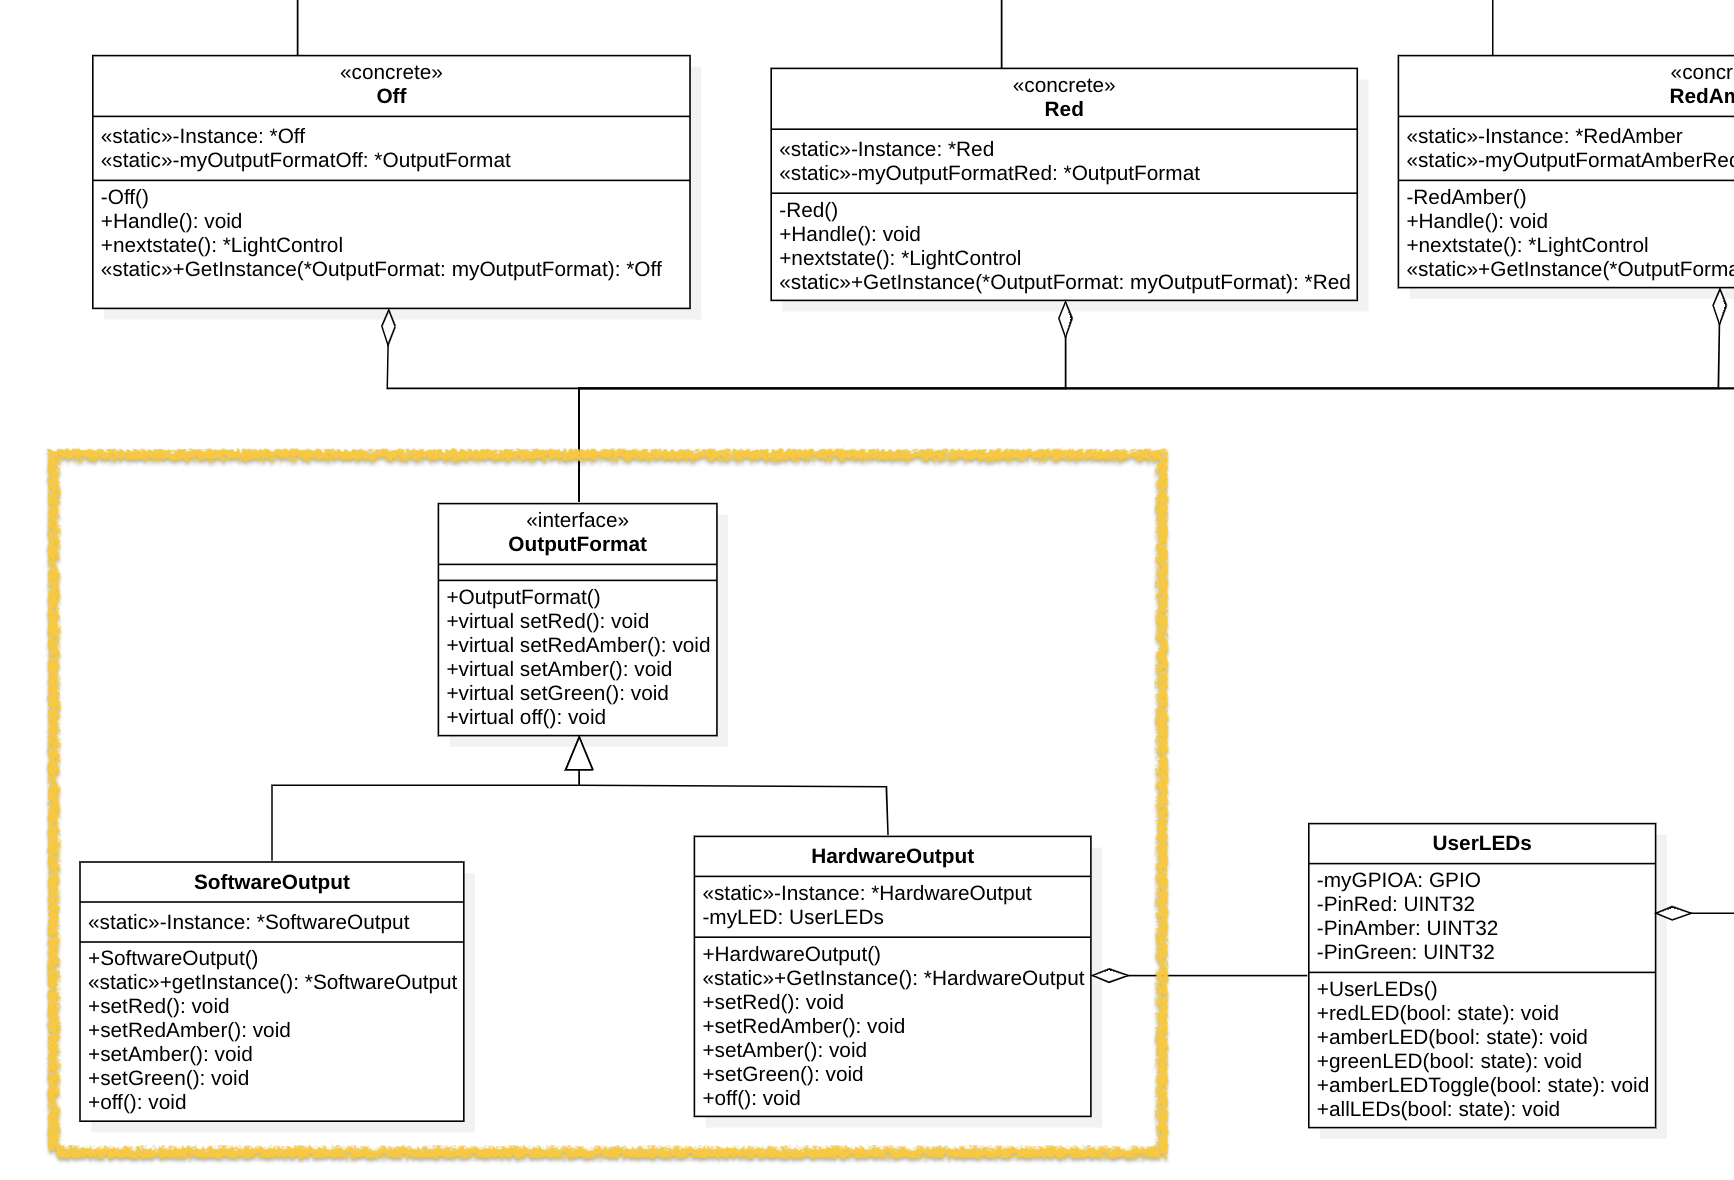
\includegraphics[width=1.0\textwidth]{images/Outputformat}
	\caption{Auszug aus dem Klassendiagramm - Ausgabeformat \protect \\ Quelle: Eigene Darstellung 
	 }
	\label{fig:output}
\end{figure}

\subsection{Eingabeformat}
\autoref{fig:input} zeigt einen Auszug aus dem Klassendiagramm, welcher für den Wechsel zwischen Hardware- und Softwareeingabe zuständig ist. 
Auch hier sind eine Interface Klasse \glqq InputFormat\grqq\: und zwei erbende Unterklassen \glqq HardwareInput\grqq\:und \glqq SoftwareInput\grqq, welche das Interface verwenden, vorzufinden. Der Wechsel zwischen Hardware- und Softwareeingabe funktioniert dabei identisch zur Logik der Hardware- und Softwareausgabe, weshalb darauf an dieser Stelle nicht weiter eingegangen wird.
\\
\begin{figure}[H] 
	\centering
	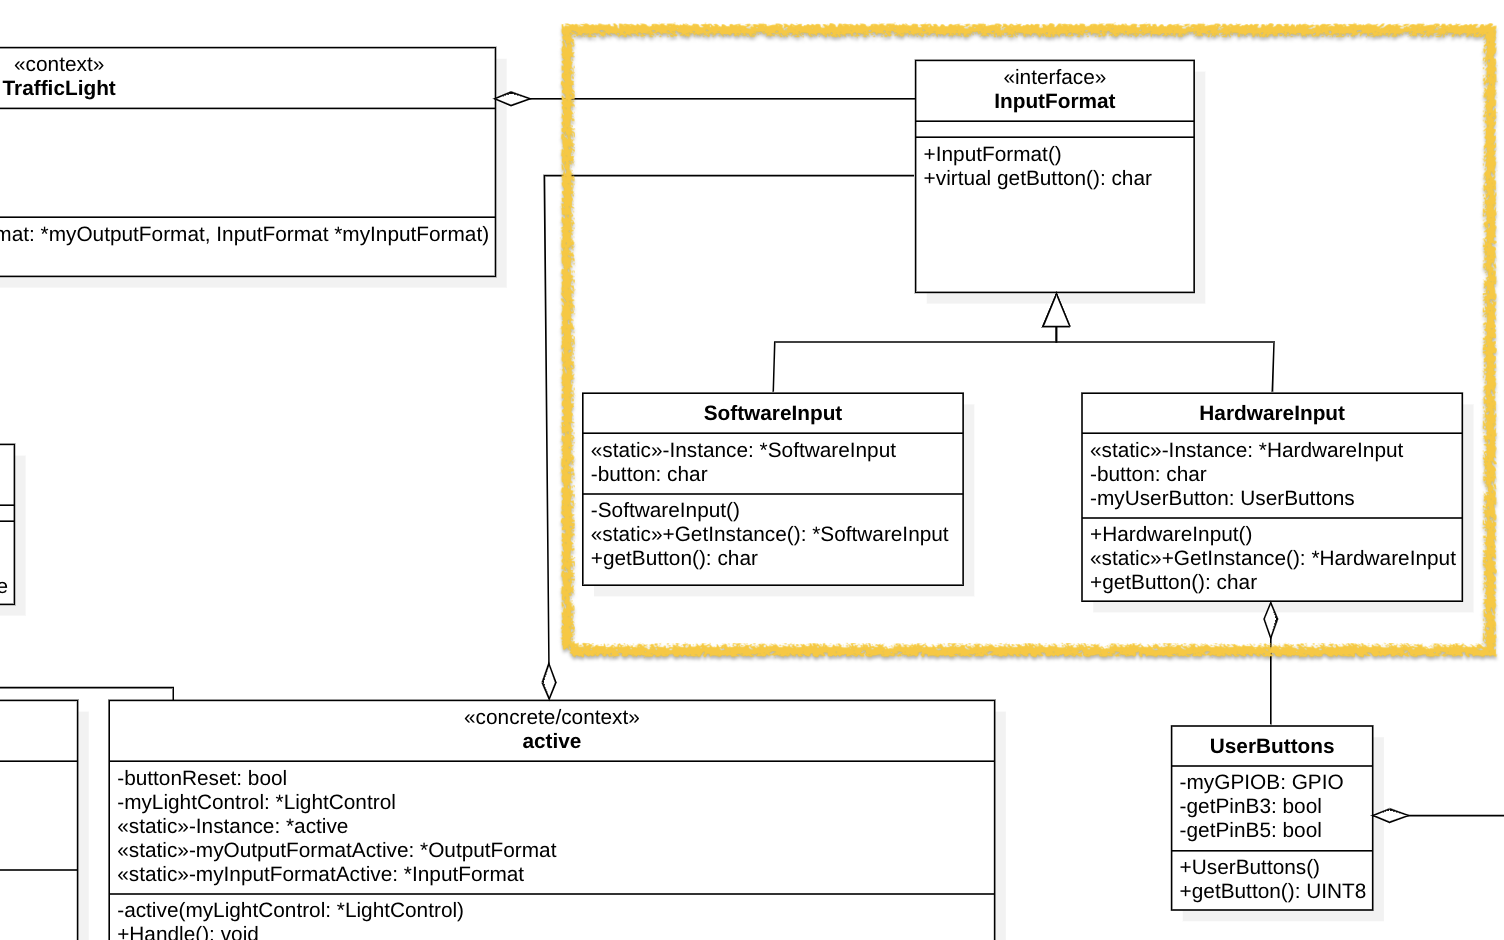
\includegraphics[width=1.0\textwidth]{images/Inputformat}
	\caption{Auszug aus dem Klassendiagramm - Eingabeformat \protect \\ Quelle: Eigene Darstellung }
	\label{fig:input}
\end{figure}

\chapter{Bedienungsanleitung}
Im Folgenden wird erläutert, wie die Ampel in der IAR Embedded Workbench zu betreiben ist. Vorausgesetzt wird, dass die Hardware per USB an den PC angeschlossen ist und die LEDs, bzw. die Taster in der richtigen Pinbelegung mit dem Board verbunden sind. Im Default Zustand geht die Ampelschaltung davon aus, dass Hardware angeschlossen ist. Wird nun das Projekt ausgeführt, so kann die Ampel über die Hardware Taster bedient werden und die Hardware LEDs leuchten entsprechend auf. Steht dem Benutzer keine Hardware zur Verfügung, so muss die Zeile „define \_HARDWAREPRESENT“ in der Main Datei auskommentiert werden. Die Ampel kann jetzt mit der Tastatur bedient werden und die Ausgabe erfolgt über das Terminal der IAR Embedded Workbench. Die Eingabe erfolgt ebenso über das Terminal des Programms. Hier kann auch die Beispiel Textdatei „Input.txt“ als Eingabe geladen werden. Die Textdatei befindet sich in den Quellcode Dateien. Die Ampel durchläuft im Beispiel zunächst alle Farbzustände im „in Betrieb“ Modus und wechselt, dann in den „außer Betrieb“ Modus. Wichtig bei der Eingabe ist, dass die Buchstaben „O“, „F“, „B“ und „X“, so eingegeben werden, als würden die entsprechenden Taster gedrückt werden. Das heißt nach jedem Buchstaben muss wieder „O“ folgen, da der Taster losgelassen wird. Auch müssen die Buchstaben öfters eingegeben werden, damit das Programm weiterläuft.


\chapter{Fazit}
Abschließend lässt sich sagen, dass die Aufgabenstellung mit dem vorliegenden Projekt erfüllt ist. Die implementierte Ampelsteuerung verfügt über alle vorgeschriebenen Funktionen. Beide definierte Betriebszustände, der „in Betrieb“ Modus und der „nicht in Betrieb“ Modus sind wie gefordert, umgesetzt. Des Weiteren kann die Ampel softwaremäßig und hardwaremäßig ausgeführt werden. Zudem sind die geforderten Methoden, Werkzeuge und Prinzipien der UML und der C++ Programmierung, die in der Vorlesung behandelt worden sind, in das Projekt eingeflossen und sinnvoll umgesetzt worden. Meiner Meinung nach hat das Projekt sehr viel Spaß gemacht und hat einen persönlich in der objektorientierten Programmierung weitergebracht. Durch das Projekt konnte eine zustandsorientierte Aufgabe objektorientiert mit der Sprache C++ umgesetzt werden.

